\chapter{Wyniki oceny eksperymentalnej}

W tej sekcji zostaną przedstawione i opisane osiągnięte wyniki. Jak już wspomniano, sport, jakim jest piłka nożna należy do dyscyplin bardzo złożonych, charakteryzującym się ogromną liczbą zmiennych, które w większości przypadków są nieprzewidywalne, trudne do uwzględnienia. W dużej części, wynik determinowany jest pewną dozą szczęścia dla jednej z drużyn. Inne czynniki są również niemożliwe do uwzględnienia. Warunki pogodowe, dyspozycja danego zawodnika oraz nastawienie każdego z graczy jest często czynnikiem kluczowym, lecz niestety niemożliwym do uchwycenia, a tym bardziej w celu wykorzystania do predykcji wyniku spotkania. Jednak istnieją również czynniki, cechy oraz atrybuty, które mają realny wpływ na wynik i właśnie je postarano się w tej pracy uchwycić oraz uwzględnić i na ich podstawie dokonywać obliczeń i zwracać rezultaty o potencjalnym zwycięzcy. Duża losowość w połączeniu z czynnikami mierzalnymi doprowadziły do wyników, które przedstawiono w poszczególnych podsekcjach dla wybranych algorytmów. Warto tutaj jeszcze wspomnieć, że zbiór danych, zanim został podzielony na zbiór uczący, walidacyjny oraz testowy, został zmniejszony w taki sposób, że najliczniejsza klasa została wyrównana do klasy mniej licznej uzyskując w ten sposób bardziej zbalansowane dane w których nie ma jednej, bardzo dominującej klasy. Metoda, do zmniejszenia danych to losowe odsianie elementów z klasy najbardziej licznej i właśnie taki zbiór został wykorzystany w dalszym etapie algorytmów. W wszystkich algorytmach próbowano również sposobu na nadlosowanie przykładów uczących metodą GlobalCS \cite{GlobalCS} i niestety w każdym z algorytmów rezultaty na wartości dokładności (\english{accuracy}) zostały zmniejszone.

\subsection{Sztuczne sieci neuronowe}
\label{SNN-results}
W tej podsekcji, przedstawione zostaną wyniki, które udało się osiągnąć dla struktury sztucznej sieci neuronowej, której parametry wraz z opisem zostały przedstawione w sekcji \ref{SNN-opis} oraz \ref{SNN-param}. Tak więc, ogólna dokładność (\english{accuracy}), obliczona na zbiorze testowym, stanowiącym 10\% z dostępnego zbioru danych wyniosła \definicja{50.79\%}, co w ogólności jest wynikiem satysfakcjonującym, ponieważ w chwili w której osoba zainteresowana predykcją zgadywała by wynik spotkania z równym prawdopodobieństwem wystąpienia jednego z trzech rezultatów, średnia trafność wyniosła by około 33\%, tak więc wartość powyżej tej liczby jest czymś więcej niż opcją zwykłego zgadywania wyniku. Dodatkowe wyliczone wartości znajdują się w tabeli \ref{tab:SNNscore}.

\begin{table}[H]
    \centering
    \caption{Wyliczone miary dla SNN}
    \label{tab:SNNscore}
    \begin{tabular}{| c | c |}
    \hline
         Precyzja (\english{precision}) &  50.41\%\\
         \hline
         Czułość (\english{recall}) &  51.06\%\\
         \hline
         Wartość Fscore &  49.78\%\\
         \hline
    \end{tabular}
\end{table}
Precyzję można interpretować jako zdarzenie w którym klasa faktycznie pozytywna została pokryta przewidywaniem pozytywnym, czułość jako zdarzenie które wskazuje w jakim procencie klasa faktycznie negatywna została pokryta przewidywaniem negatywnym, a fscore interpretuje się jako ważoną średnią harmoniczną precyzji i czułości. Miary te zostały obliczone jako nieważona średnia dla każdej wartości dla poszczególnej klasy. Dodatkowo macierz pomyłek przedstawia się następująco:

\begin{center}
\begin{table}[H]
\renewcommand{\arraystretch}{1.5}
\caption{Macierz pomyłek dla SNN}
\label{tab:macierzSNN}
\begin{center}
\begin{tabular}{|c|c|c|c|c|}
   \cline{3-5} 
   \multicolumn{1}{c}{} & & \multicolumn{3}{c|}{Predicted} \\ \cline{3-5}
   \multicolumn{1}{c}{} & & Draw & HomeWin & AwayWin \\ \hline
   
   {Observed/actual}
   & Draw & 20 & 23 & 22 \\ \cline{2-5}
   & HomeWin & 12 & 37 & 10  \\ \cline{2-5}
   & AwayWin & 10 & 17 & 40 \\ \hline
\end{tabular}
\end{center}
\end{table}
\end{center}
Można zauważyć, że najwięcej błędów popełnianych w predykcji, jest w momencie, kiedy faktyczna klasa symbolizuje remis pomiędzy drużynami. Problem ten mógł wynikać z powodu wyrównanych statystyk, które jednak nie były na tyle podobne by określić je jako te dające remis, lecz przeważyły na jedną ze stron, a jak wiadomo, nie tylko dane statystyczne to kluczowy czynnik w sporcie. Remis oznacza również wynik bezbramkowy czyli sytuację, w której potencjalnie gorsza drużyna bardzo dobrze się broniła i udało jej się nie stracić bramki - takie taktyki są również obecne w rozgrywkach sportowych i można to podać jako jeden z powodów dla których właśnie predykcja remisów wypadła najmniej skutecznie.
Po procesie nauki postanowiono sprawdzić wpływ danych cech wejściowych na predykcję danego wyniku i odkryć, które atrybuty lub kombinacje cech dla sztucznej sieci neuronowej odgrywały kluczowe role i najbardziej przyczyniły się do predykcji konkretnego wyniku. Dokonaliśmy tego przy użyciu wartości Shapleya \cite{shapley} oraz biblioteki w języku Python \definicja{Shap} \cite{NIPS2017_7062}.
\begin{figure}[H] 
        \centering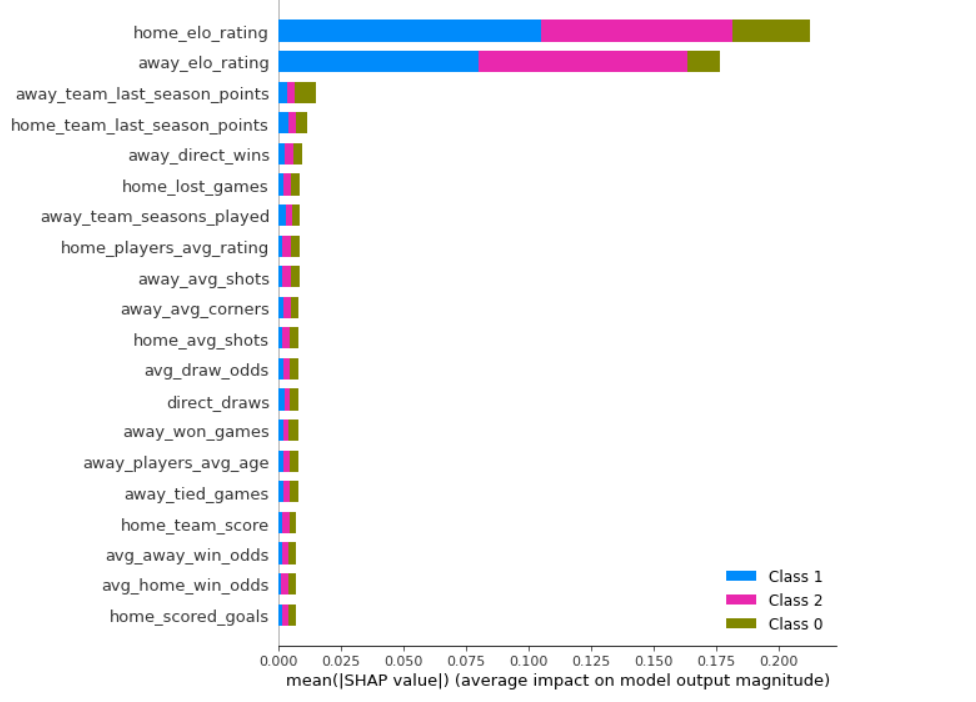
\includegraphics[width=10cm,height=6cm]{figures/ShapSNN.png}
        \caption{Wartości Shapleya dla SNN}\label{Shap-SNN}
\end{figure}
Jak można zauważyć na rysunku \ref{Shap-SNN}, atrybut \textit{home\_elo\_rating} oraz \textit{away\_elo\_rating} miały największe znaczenie i wagę, które w największym stopniu wpływa na wyniki predykcji sieci. Nie jest to zaskakujący rezultat, ponieważ atrybut ten jest odzwierciedleniem ogólnej siły drużyny w danym meczu oraz aktualizowany jest co spotkanie więc można było się spodziewać o dużym znaczeniu tej cechy. Dodatkowo, warto zauważyć, że cecha określająca ilość punktów w zeszłych sezonach danej drużyny również była dość znacząca (choć nieporównywalnie mniej niż wartości elo\_rating) i można ją zinterpretować jako dotychczasowy sposób radzenia sobie danej drużyny w analizowanej lidze.

\subsection{Maszyny wektorów nośnych}
Ta sekcja będzie prezentować wyniki dla algorytmu SVM. Dokładność (\english{accuracy}) na 10-cio procentowym zbiorze testowym (takim samym jak poprzednio) wyniosła 49.74\%. Dodatkowe miary, które interpretuje się również tak samo jak w podsekcji \ref{SNN-results}, wyglądają następująco:

\begin{table}[H]
    \centering
    \caption{Wyliczone miary dla SVM}
    \label{tab:SVMscore}
    \begin{tabular}{| c | c |}
    \hline
         Precyzja (\english{precision}) &  48.79\%\\
         \hline
         Czułość (\english{recall}) &  49.90\%\\
         \hline
         Wartość Fscore &  48.45\%\\
         \hline
    \end{tabular}
\end{table}
Dodatkowo, macierz pomyłek została przedstawiona w tabeli \ref{tab:macierzSVM}
\begin{center}
\begin{table}[H]
\renewcommand{\arraystretch}{1.5}
\caption{Macierz pomyłek dla SVM}
\label{tab:macierzSVM}
\begin{center}
\begin{tabular}{|c|c|c|c|c|}
   \cline{3-5} 
   \multicolumn{1}{c}{} & & \multicolumn{3}{c|}{Predicted} \\ \cline{3-5}
   \multicolumn{1}{c}{} & & Draw & HomeWin & AwayWin \\ \hline
   
   {Observed/actual}
   & Draw & 18 & 21 & 26 \\ \cline{2-5}
   & HomeWin & 13 & 35 & 11  \\ \cline{2-5}
   & AwayWin & 10 & 15 & 42 \\ \hline
\end{tabular}
\end{center}
\end{table}
\end{center}
Również przy użycia tego klasyfikatora, prawidłowa predykcja remisu jest najgorzej realizowana. Predykcja zwycięstw oraz porażek jest dużo bardziej skuteczna, a wytłumaczenie tego faktu może być podobne jak w podsekcji \ref{SNN-results}. Również tutaj wykorzystano wartości Shapleya \cite{shapley} oraz biblioteki w języku Python \definicja{Shap} \cite{NIPS2017_7062} w celu określenia, które kombinacje cech miały największy wpływ na otrzymywany wynik w naszym algorytmie.

\begin{figure}[H] 
        \centering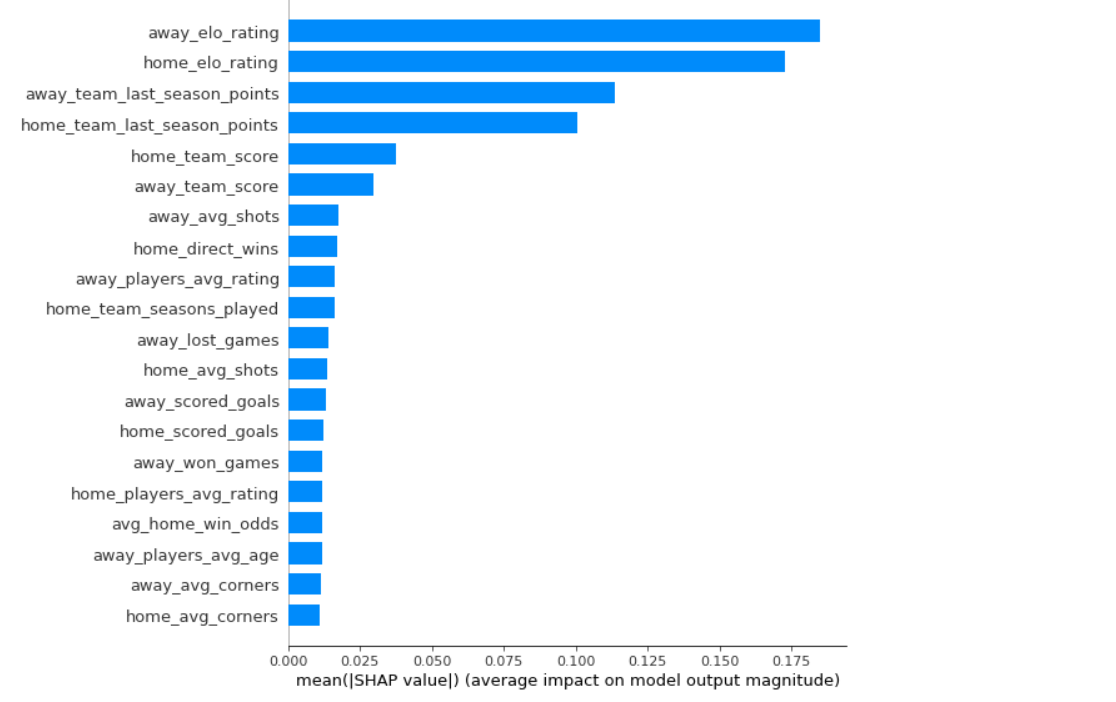
\includegraphics[width=10cm,height=6cm]{figures/ShapSVM.png}
        \caption{Wartości Shapleya dla SVM}\label{Shap-SVM}
\end{figure}
W tym przypadku, również wartości elo\_rating odgrywały kluczową rolę dla algorytmu SVM ponieważ wartość ta to zagregowana i wyliczona wartości siły i zdolności danej drużyny czyli mająca realny wpływ na to, jak dana drużyna ma aktualnie predyspozycje oraz zdolności. Tutaj również dużą wartość przyjęły atrybuty takie jak ilość punktów danych drużyn w poprzednim sezonie oraz ilość punktów danej drużyny w aktualnie rozgrywanym sezonie. Wszystkie te czynniki, oraz dobór parametrów dały rezultaty jak przedstawiono powyżej.